\begin{center}
\textbf{Заключение}
\end{center}

  В ходе курсового проекта был проведен общетехнический анализ
  беспроводного роутера ассиметричной цифровой абонентской линии
  ASW800 ADSL.

  Были выполнены расчеты теплового режима РЭС в
  герметичном корпусе,
  в герметичном корпусе с внутренним перемешиванием,
  в герметичном корпусе с наружным обдувом,
  в герметичном оребренном корпусе,
  в перфорированном корпусе,
  и при принудительно воздушном охлаждении
  для процессора TNETD7300.

  Температуры элемента принадлежат рабочему диапазону
  температур. Сами по себе значения температур
  адекватны, однако результаты расчетов можно подставить под сомнение.

  Выполнен анализ и обработка полученных результатов расчета и
  моделирования теплового режима РЭС.

  Выполнение общетехнического анализа, расчетов теплового
  режима РЭС и анализ с обработкой полученных результатов
  подтверждае правильный выбор производителем системы охлаждения.
  Значительные изменения конструкции и способа охлаждения невыгодны.

  Таким образом большая часть целей и задач курсового проекта,
  была реализована.

  \newpage



% \bibligoraphystyle{5sem}
% \renewcommand{\bibsection}{{Cписок использованных источников}}
\renewcommand{\refname}{\textbf{Cписок использованных источников}}
\DeclareFieldFormat{url}{Режим доступа\addcolon\space\url{#1}}
\DeclareFieldFormat{title}{{#1}}
\DeclareFieldFormat{labelnumberwidth}{[{#1}]\adddot  }
\printbibliography

\newpage
\begin{center}
\textbf{Приложение А}\\
\textbf{Обязательное}\\
\textbf{Параметры компонентов}
\end{center}

Рассеиваемая мощность процессора TNETD7300 0,525Вт.

Площадь поверхности 0.000473 $\mathrm{м^2}$.


Длина корпуса 14см.

Ширина корпуса 10 см.

Высота корпуса 3 см.
\newpage


\begin{center}
\textbf{Приложение Б}\\
\textbf{Обязательное}\\
\textbf{Отчет о проверке на заимствования в системе «Антиплагиат»}

\begin{figure}[h]
  \centering
  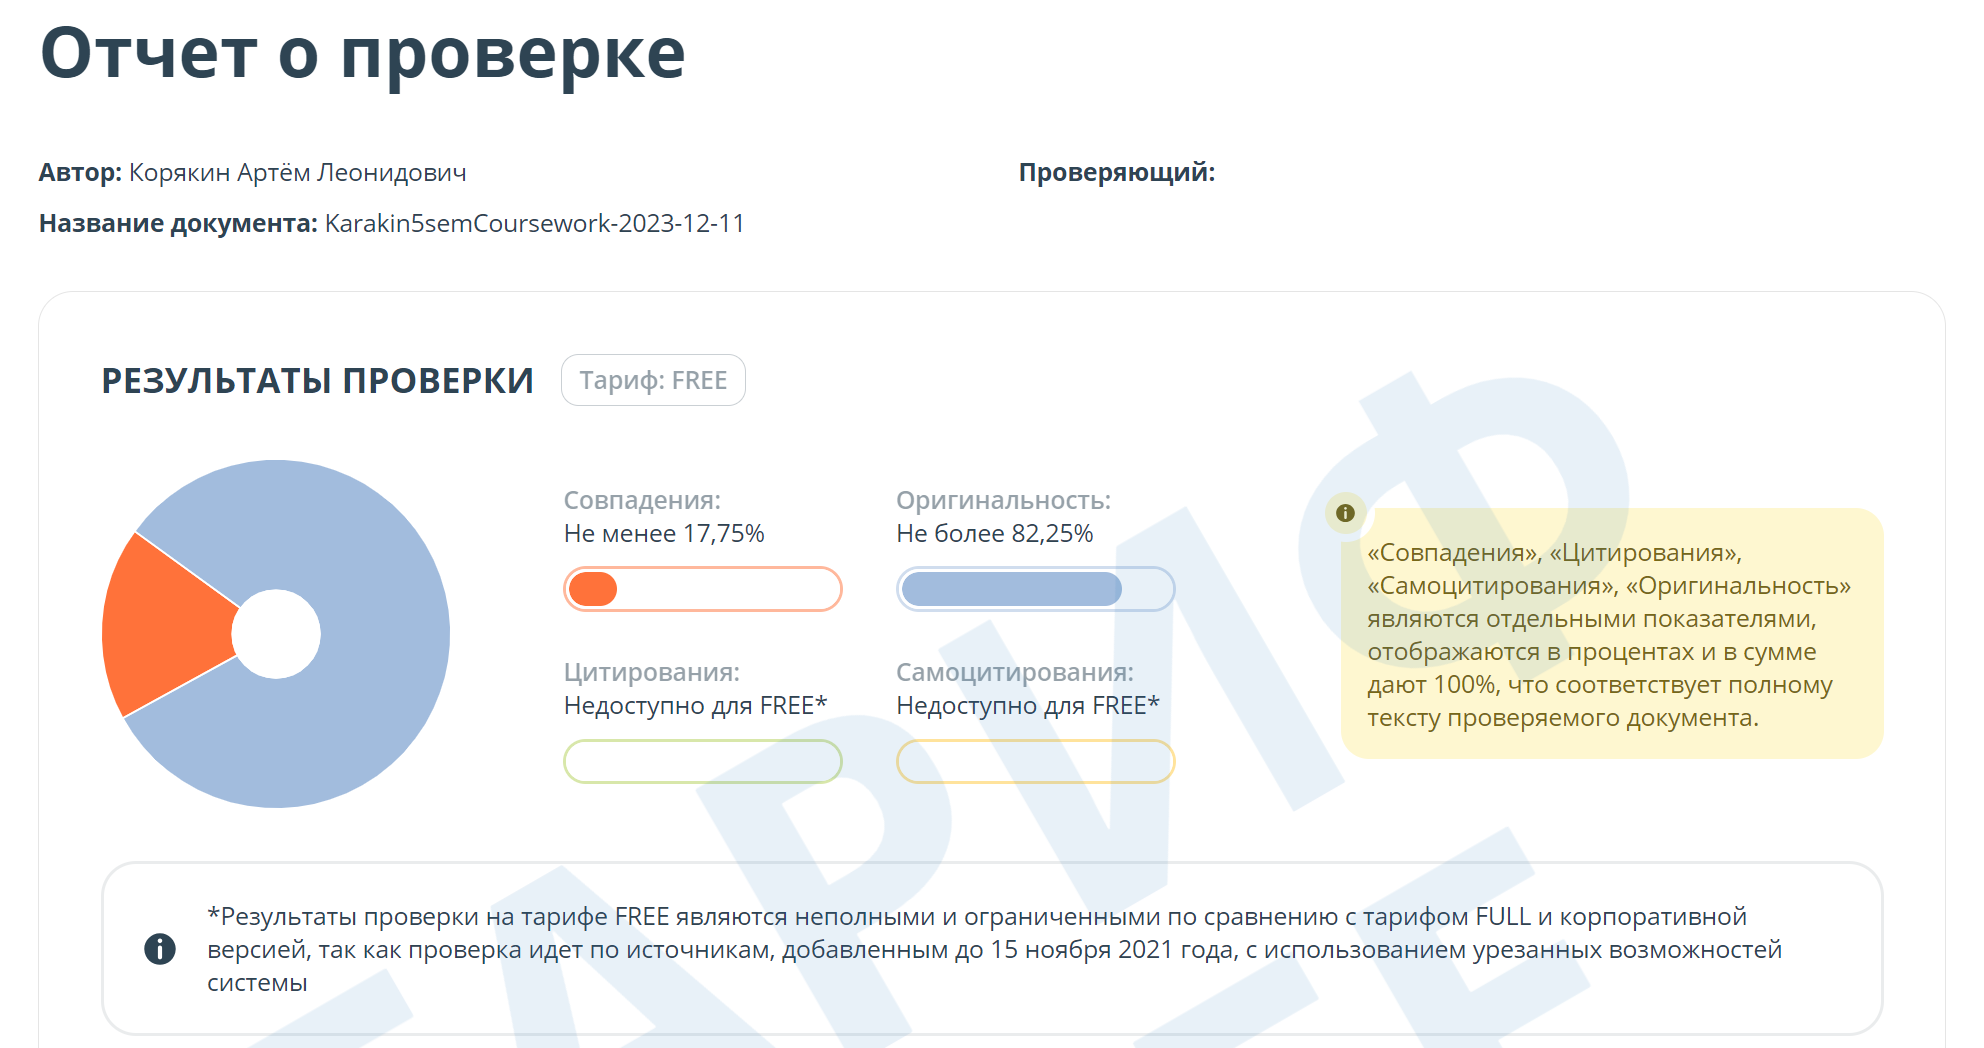
\includegraphics[scale = 0.5]{images2/antiplagiat01.png}
  \caption{
    Результат проверки на заимствования в системе «Антиплагиат»}
\end{figure}

\begin{figure}[h]
  \centering
  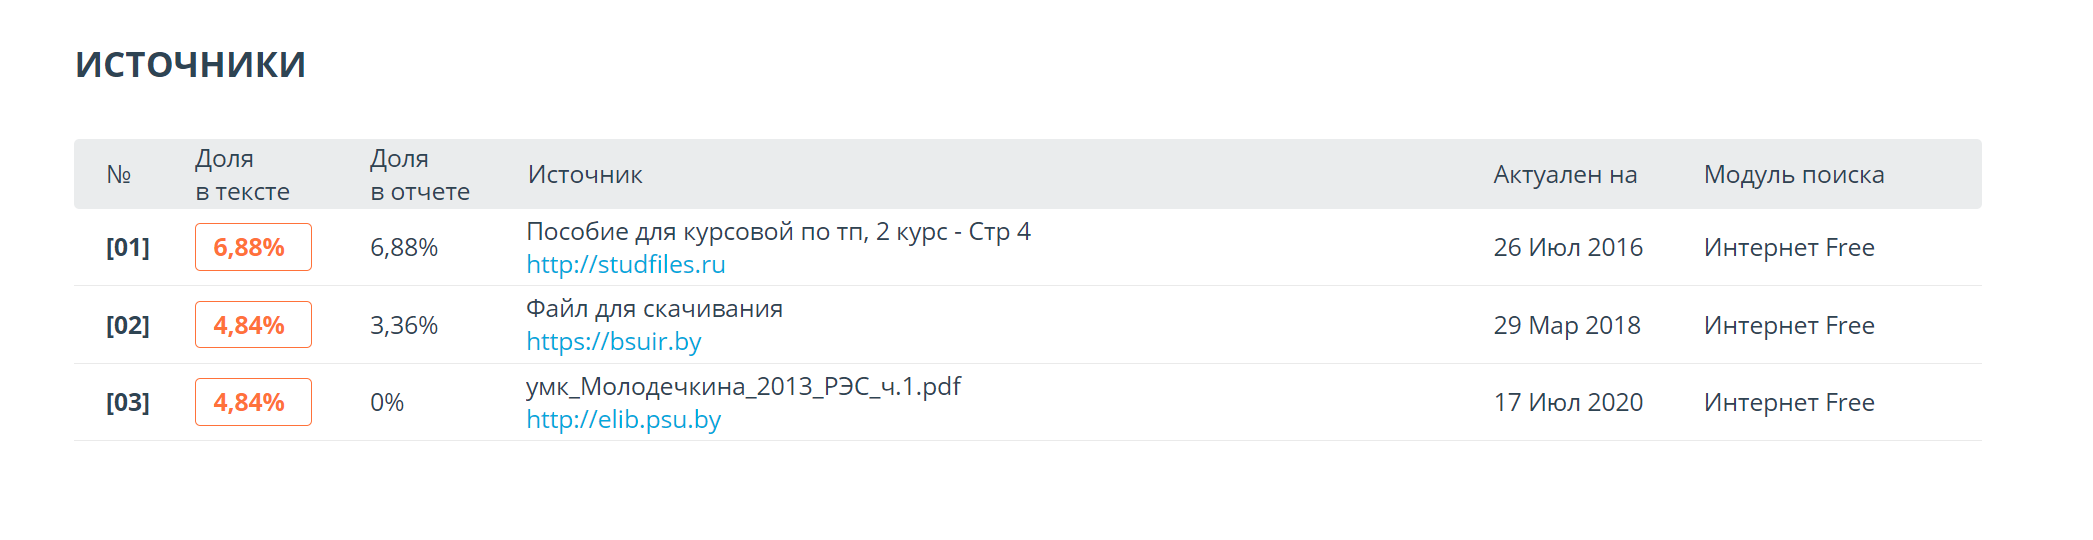
\includegraphics[scale = 0.5]{images2/antiplagiat02.png}
  \caption{ Источники, найденные при проверке в системе «Антиплагиат»}
\end{figure}


\end{center}
